\documentclass{article}

% amsmath must come before arxiv.sty: both define \And, and the author block needs the arxiv.sty version
\usepackage{amsmath}
\usepackage{amssymb}
\usepackage{arxiv}

\usepackage[utf8]{inputenc}
\usepackage[T1]{fontenc}
\usepackage{hyperref}
\usepackage{url}
\usepackage{booktabs}
\usepackage{amsfonts}
\usepackage{nicefrac}
\usepackage{microtype}
\usepackage{graphicx}
\usepackage{tabularx}
\usepackage{xcolor}
\usepackage{enumitem}
\usepackage{algorithm}
\usepackage{algpseudocode}
\setlist{nosep,leftmargin=*}
\graphicspath{{figures/}}
\newcolumntype{L}{>{\raggedright\arraybackslash}X}
\newcommand{\Bref}{B_{\mathrm{ref}}}
\newcommand{\RF}{\mathrm{RF}}

\title{The Last Rescue: Learning to Cooperate Under Resource Scarcity}

\author{
  Kshitij Suresh Giri\\
  Indian Institute of Technology Gandhinagar\\
  Gandhinagar, India\\
  \texttt{23110177}
  \And
  Panjari Maheshkumar Patel\\
  Indian Institute of Technology Gandhinagar\\
  Gandhinagar, India\\
  \texttt{23110236}
  \AND
  DV Snehal\\
  Indian Institute of Technology Gandhinagar\\
  Gandhinagar, India\\
  \texttt{23110083}
  \And
  Kshitish Madbhavi\\
  Indian Institute of Technology Gandhinagar\\
  Gandhinagar, India\\
  \texttt{24110175}
}

\date{}
\renewcommand{\shorttitle}{The Last Rescue}
\renewcommand{\headeright}{}
\renewcommand{\undertitle}{}

\begin{document}
\maketitle

\begin{abstract}
We study how resource scarcity affects the ability of independently learning agents to learn cooperative rescue.
\emph{The Last Rescue} is a partially observed $10\times10$ grid in which three agents with private, non-refillable
budgets search for six victims; half are \emph{heavy} and need one agent to RESCUE while a second ASSISTs on the same
cell in the same step. Scarcity $\rho$ is a fraction of a calibrated just-enough budget ($\Bref=64$, horizon $H=105$),
giving 64, 32, 19 and 13 units per agent. Agents learn with independent tabular Q-learning (IQL) and are compared with
random, greedy and hand-designed cooperative policies and a full-information oracle, over 10 training seeds per
condition. Scarcity lowers the rescue fraction monotonically from $0.573$ to $0.087$ (Friedman $p=1.4\times10^{-6}$,
every seed in the same direction), and heavy, cooperation-requiring rescues fall fastest ($0.422\to0.016$).
Interventions show that coordination learned with teammates matters at every level, but a world with only light victims
loses \emph{more} rescue-fraction points under scarcity, so the decline is not specific to cooperation. Seven
additional experiments that each change one design choice keep the decline.
\end{abstract}

\keywords{Multi-Agent Reinforcement Learning \and Independent Q-Learning \and Search and Rescue \and Resource Scarcity
\and Cooperation \and Partial Observability}

% =====================================================================================================================
\section{Introduction}
% =====================================================================================================================
Multi-agent search and rescue needs agents to divide the search area, help one another and spend limited resources
well; uncoordinated agents duplicate search and waste resources~\cite{shoham2008,queralta2020}. Scarcity sharpens this:
an agent that spends its budget exploring may later be unable to provide the help a teammate needs. Reinforcement
learning can acquire such behaviour, but independent learners face a non-stationary problem because their teammates
learn at the same time~\cite{zhang2021,tan1993}. Related work has studied cooperation and competition for resources in
sequential multi-agent settings~\cite{leibo2017} and learning-based disaster response and search and
rescue~\cite{nguyen2018,hickling2026}. Our question is:
\begin{center}
\emph{How does resource scarcity affect the ability of autonomous agents to learn cooperative rescue strategies?}
\end{center}
We vary only the budget and keep the environment generator, learning algorithm, reward, training budget and evaluation
fixed. The contributions are a tested environment with exact budget, feasibility and information rules; a calibration
that gives $\rho$ a defined meaning across map sizes; a study with hypotheses fixed before any learning run; interventions
that separate cooperation from other effects of scarcity; and a public pipeline that regenerates every reported number.

% =====================================================================================================================
\section{Preliminaries}
% =====================================================================================================================
A finite-horizon Markov game
$\mathcal{G}=\langle N,S,(A_i),P,(R_i),(O_i),H\rangle$ has agents $N=\{1,\dots,n\}$ that act simultaneously; the joint
action $\mathbf{a}_t$ drives $s_{t+1}\sim P(\cdot\mid s_t,\mathbf{a}_t)$, agent $i$ receives $r^i_t$ and sees only
$o^i_t=O_i(s_t)$~\cite{shoham2008}. In independent Q-learning each agent learns its own table~\cite{watkins1992,sutton2018}
\begin{equation}
Q_i(o_t,a_t)\leftarrow Q_i(o_t,a_t)+\alpha\Big[r^i_t+\gamma(1-d_t)\max_{a'\in\mathcal{M}_i(o_{t+1})}Q_i(o_{t+1},a')-Q_i(o_t,a_t)\Big],
\end{equation}
where $\mathcal{M}_i$ is the set of valid actions and $d_t$ marks termination, and treats teammates as part of the
environment~\cite{tan1993}. Because teammates also learn, what each agent experiences changes over time and the
single-agent convergence guarantee is lost. A drop in performance under scarcity may therefore come from less
cooperation, noisier learning or fewer learning steps; Section~\ref{sec:attr} separates these.

% =====================================================================================================================
\section{Problem Formulation}
% =====================================================================================================================
\paragraph{Environment and actions.} The map is a $10\times10$ grid with 15\% walls, hazard cells on 10\% of free cells
(entering costs 2), a base where all agents start, and $V=6$ victims at Chebyshev distance $\ge2$ from the base, exactly
3 of them heavy. The state is $s_t=(M,V_t,X_t,B_t,t,D_t)$: map, victim status, positions, budgets, time and each
agent's memory. Actions and costs are in Table~\ref{tab:actions}. A heavy victim is rescued only when one agent RESCUEs
and another ASSISTs on its cell in the same step; two RESCUEs fail and both pay.

\begin{table}[h]
\centering\small
\caption{Actions, integer costs and validity (checked on the agent's own observation).}
\label{tab:actions}
\begin{tabularx}{\linewidth}{@{}lcL@{}}
\toprule
Action & Cost & Valid when \\
\midrule
UP, DOWN, LEFT, RIGHT & 1 (2 into hazard) & target is not a wall and the agent can pay \\
SEARCH & 2 & always (reveals victims within Chebyshev radius 2) \\
RESCUE & 3 & the agent stands on a victim it sees as waiting \\
ASSIST & 2 & on a heavy victim with a teammate on the same cell \\
WAIT & 0 & always \\
\bottomrule
\end{tabularx}
\end{table}

\paragraph{Budgets, exhaustion and feasibility.}\label{sec:budget} Each agent owns a private, non-transferable budget
$B^i_0=\mathrm{round}(\rho\Bref)$ with $B^i_{t+1}=B^i_t-c(a^i_t)$; an action is valid only if $c(a)\le B^i_t$, so
budgets never become negative. A pooled team budget $nB_0$ is studied as an ablation. An episode ends at the first of:
\emph{all rescued}; \emph{exhausted}, $\max_i B^i_t<c_R$, so no rescue is possible any more; or the \emph{horizon}
$t=H$. An agent with $B^i_t<1$ is \emph{dormant} (only WAIT is valid). An instance is \emph{feasible} if at least one
victim can be rescued within the budgets and horizon (exact check); maps infeasible at the hardest level were
regenerated before freezing (1.0\% of test maps).

\paragraph{Reward and objective.}
$R^i_t=\lambda_I r^i_{\mathrm{ind},t}+\lambda_T r_{\mathrm{team},t}-\lambda_C c(a^i_t)$ with $\lambda_I=\lambda_T=1$,
$\lambda_C=0.02$. $r_{\mathrm{ind}}$ pays 0.1 for discovering a victim, 1.0 for a light rescue and 0.5 each to the
rescuer and assister of a heavy victim; $r_{\mathrm{team}}$ pays 1.0 to every agent per rescue by anyone. Coefficients
are identical at every $\rho$. Each agent maximises $J_i=\mathbb{E}[\sum_{t<H}\gamma^t R^i_t]$; the team outcome is the
rescue fraction $\RF$ (rescued / $V$).

\paragraph{Observation.} Each agent observes a discrete tuple $o=(f_1,\dots,f_5)$ with $3{,}960$ values: $f_1$ the
nearest victim it believes unrescued (none, here-light, here-heavy, or first step of the cheapest path $\times$
near/far); $f_2$ the first step towards the nearest never-observed cell; $f_3$ the nearest teammate within radius 3
(none, same cell, direction); $f_4$ its budget bucket with thresholds $(3,16,32)$; $f_5$ the elapsed third of the
horizon. Features use only the agent's own memory and view; a victim rescued out of view stays in memory until seen.

% =====================================================================================================================
\section{Methodology}
% =====================================================================================================================
\subsection{Environment implementation}
One step executes payment, simultaneous moves, RESCUE/ASSIST resolution, observation, reward, dormancy and termination;
every submitted action is re-validated against the mask. The environment is deterministic given the actions (about
$29\,\mu$s per agent-step) and covered by 269 automated tests. Maps come from frozen, disjoint seed lists: 1{,}000
training, 50 validation (checkpoints only), 100 test and 100 shifted-test maps (25\% walls, more victims).

\subsection{Calibrating the budget scale}\label{sec:calib}
All rules were fixed before the first calibration run and applied to 200 separate calibration maps.
(1)~\emph{Horizon:} with unlimited budget, the cooperative baseline needs $T_{90}=73$ steps (90th percentile) to rescue
90\% of victims; $H=\lceil T_{90}/0.7\rceil=105$, so time does not bind a competent team.
(2)~\emph{Reference budget:} $\Bref=64$ is the 90th percentile of that baseline's per-agent consumption.
(3)~\emph{Levels:} $\rho$ is chosen where the cooperative baseline's $\RF$ is nearest 0.70 (Moderate), 0.40 (Scarce)
and 0.10--0.15 (Critical), with at least 95\% of maps feasible; $\rho=0.1$ is feasible on only 33\%, so Critical is
$\rho=0.2$. The result is $\rho=1.0/0.5/0.3/0.2$, i.e.\ 64/32/19/13 units (Fig.~\ref{fig:calib}). Below Abundant,
94--100\% of cooperative episodes end by exhaustion, so these levels are budget-limited, not time-limited. Recalibrating
five other configurations ($L\in\{8,12\}$, two victim densities, an all-light world) with the same rules gives the same
cooperative $\RF$ per level within 0.08 for $L\ge10$, so $\rho$ is comparable across map size and density there.

\begin{figure}[t]
\centering
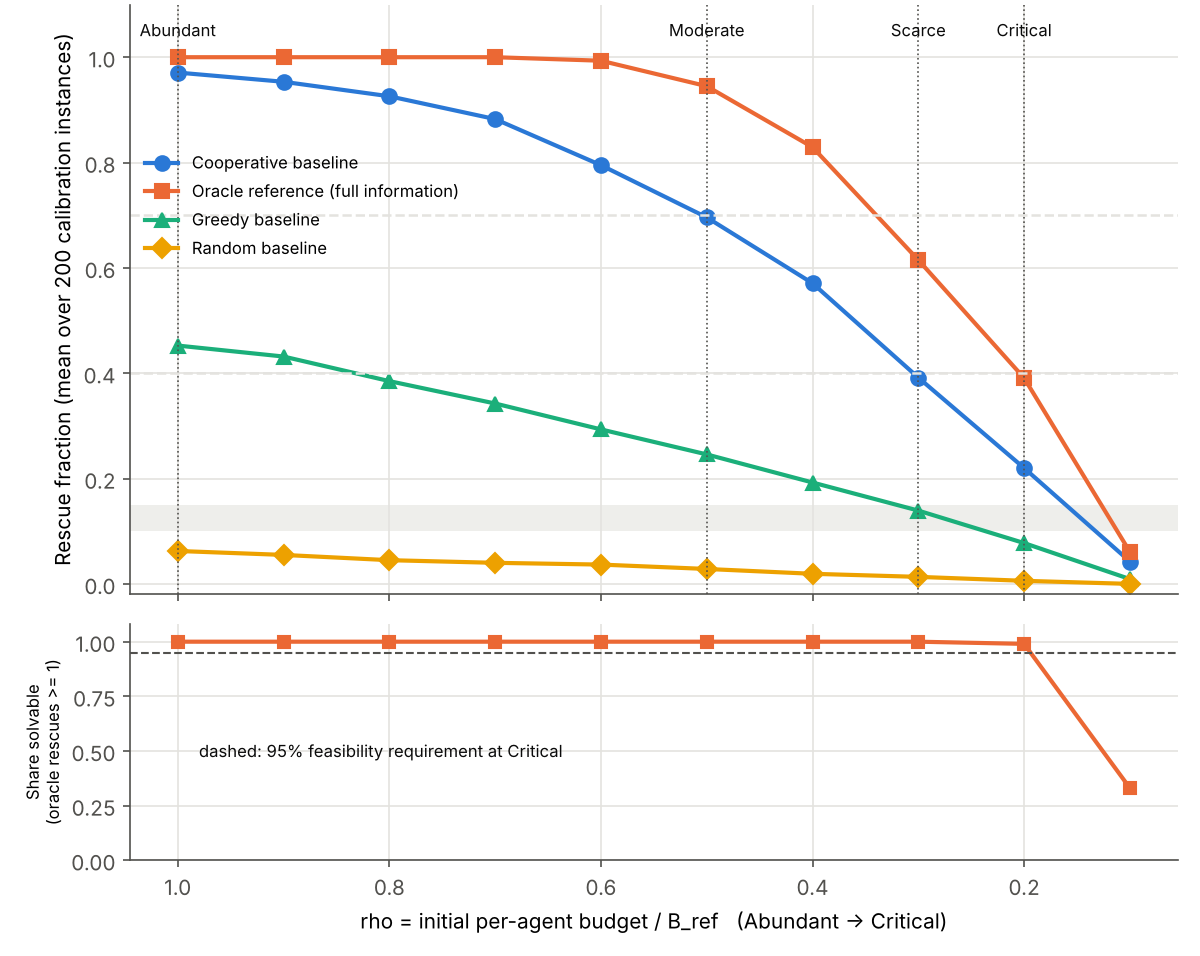
\includegraphics[width=0.5\linewidth]{fig_cal_main.png}
\caption{Calibration on 200 calibration maps. Top: rescue fraction of each reference policy against $\rho$ (dotted
lines: selected levels). Bottom: share of feasible maps.}
\label{fig:calib}
\end{figure}

\subsection{Independent Q-learning}
Each agent has its own table $Q_i\in\mathbb{R}^{3960\times8}$, initialised to 0 (Algorithm~\ref{alg:iql}). Actions are
$\epsilon$-greedy over valid actions with random tie-breaking. Hyperparameters were fixed in advance and a pilot on
validation maps confirmed learnability without changing them: $\alpha=0.1$, $\gamma=0.98$, $\epsilon$ decays linearly
from 1.0 to 0.05 over the first 70\% of 8{,}000 episodes.

\begin{algorithm}[h]
\caption{IQL training for one run (seed $s$, budget level $\rho$)}
\label{alg:iql}
\begin{algorithmic}[1]
\State $Q_i\gets 0$ for all agents; map order and exploration streams from seed $s$
\For{episode $e=1..8000$}
  \State reset on the next training map with $B^i_0=\mathrm{round}(\rho\Bref)$
  \While{not terminated}
    \State each agent: random valid action w.p.\ $\epsilon(e)$, else $\arg\max_{a\in\mathcal{M}_i(o^i)}Q_i(o^i,a)$
    \State step; observe $R^i$, $o'^i$, $\mathcal{M}_i(o'^i)$, done $d$
    \State for each non-dormant agent: $Q_i(o^i,a^i)\mathrel{+}=\alpha[R^i+\gamma(1-d)\max_{a'}Q_i(o'^i,a')-Q_i(o^i,a^i)]$
  \EndWhile
  \State every 500 episodes: greedy evaluation on validation maps ($\RF$, cooperation metrics, policy churn)
\EndFor
\end{algorithmic}
\end{algorithm}

\subsection{Baselines and oracle}
All baselines are decentralised and use the same observations. \textbf{Random} picks a valid action. \textbf{Greedy}
walks to the nearest affordable victim, rescues lights, tries each heavy victim once and never ASSISTs (its identical
agents tend to move in lockstep, so it represents uncoordinated rather than optimally selfish agents).
\textbf{Cooperative} splits the map into sectors, waits at heavy victims for help, walks to teammates that stay put,
and uses a fixed role convention (lowest index RESCUEs). The \textbf{oracle} sees the full state and plans centrally by
greedy route insertion (99\% optimal on 300 small instances); it shows what the budget allows and is not a learner.

\subsection{Cooperation metrics}\label{sec:metrics}
Team reward cannot show cooperation, since selfish agents that each rescue lights also earn it, so we measure
cooperation from the action logs (Table~\ref{tab:metrics}). Ratio metrics are pooled per seed over the 100 test
episodes. Each metric was checked on scripted episodes with known answers before any learning (42/45 checks passed;
the failures show that PSS largely tracks reward, so it is not used as independent evidence of cooperation).

\begin{table}[h]
\centering\small
\caption{Cooperation metrics (cooperative direction in brackets).}
\label{tab:metrics}
\begin{tabularx}{\linewidth}{@{}llL@{}}
\toprule
C1 & Effective assist rate EAR & heavy rescues / ASSIST actions (higher) \\
C2 & Redundant search RSR & share of SEARCHes whose area is $\ge50\%$ already covered, by others for RSR$_{\text{other}}$ (lower) \\
C3 & Territory division TDI & $1-$ mean pairwise Jaccard overlap of the agents' visited cells (higher) \\
C4 & Productive spend PSS; Gini & minimal cost of completed rescues / budget spent (higher); Gini of spending (lower) \\
C5 & Cooperation rate CR & share of non-WAIT actions that are part of a heavy rescue or converge on one (higher) \\
\bottomrule
\end{tabularx}
\end{table}

\subsection{Attribution design}\label{sec:attr}
A correlation between scarcity, cooperation and rescues does not show that cooperation is the mechanism, so we
intervene, always on the same seeds and test maps: \textbf{A1} mismatched teams (agents of different seeds deployed
together); \textbf{A2} one agent replaced by a random or WAIT-only agent; \textbf{A3} an all-light world with the same
maps and budgets, where no victim needs a partner (difference-in-differences of the scarcity effect); \textbf{A4} agents
trained alone and deployed together; \textbf{A5} policy churn and TD error as direct measures of non-stationarity;
\textbf{A6} lower levels trained for as many environment steps as Abundant, because scarce episodes are shorter.

\subsection{Protocol and statistics}
Seven hypotheses were fixed before the first learning run: H0 IQL beats random at Abundant; H1 $\RF$ changes with
$\rho$; H2 cooperation metrics change with $\rho$; H3 IQL differs from each baseline; H4 original teams beat
mismatched teams (A1); H5 the scarcity effect differs in the all-light world (A3); H6 joint training beats solo
training (A4). Each condition has 10 training seeds, and seed $s$ uses the same map order, exploration stream and test
maps in every condition, so conditions are compared within seed; the seed (mean over 100 test maps) is the unit of
analysis. We use Friedman~\cite{friedman1937} and Page trend~\cite{page1963} tests across levels, Wilcoxon
signed-rank~\cite{wilcoxon1945} tests for pairs, Holm correction within each hypothesis family~\cite{holm1979}
($\alpha=0.05$), and 95\% bootstrap CIs over seeds~\cite{efron1979}. In total 350 runs were trained (4.5 CPU-hours).

\paragraph{Assumptions.} The static map is known in advance, so $f_1$ and $f_2$ give planner directions and the learner
does not learn navigation; there is no communication; two agents on a heavy victim see the same observation, so roles
are not signalled; the reward favours light victims for a selfish agent (2.0 vs 1.5 per agent); Q-values start at 0
and WAIT is free; dormant agents do not learn; the budget buckets are absolute; and $\Bref$ is defined by a
hand-designed policy. Section~\ref{sec:robust} tests the choices that can be varied.

% =====================================================================================================================
\section{Results}
% =====================================================================================================================
\subsection{Learnability (H0, A5)}
IQL learns: at Abundant all 10 seeds rescue more than random ($0.573$ vs $0.063$; $p=9.8\times10^{-4}$). Learning
starts late and is still changing at 8{,}000 episodes (Fig.~\ref{fig:learning}): none of the 40 main runs meets the
stability criterion (policy churn $<5\%$ and validation $\RF$ range $<0.02$), so all results describe policies after a
fixed training budget.

\begin{figure}[h]
\centering
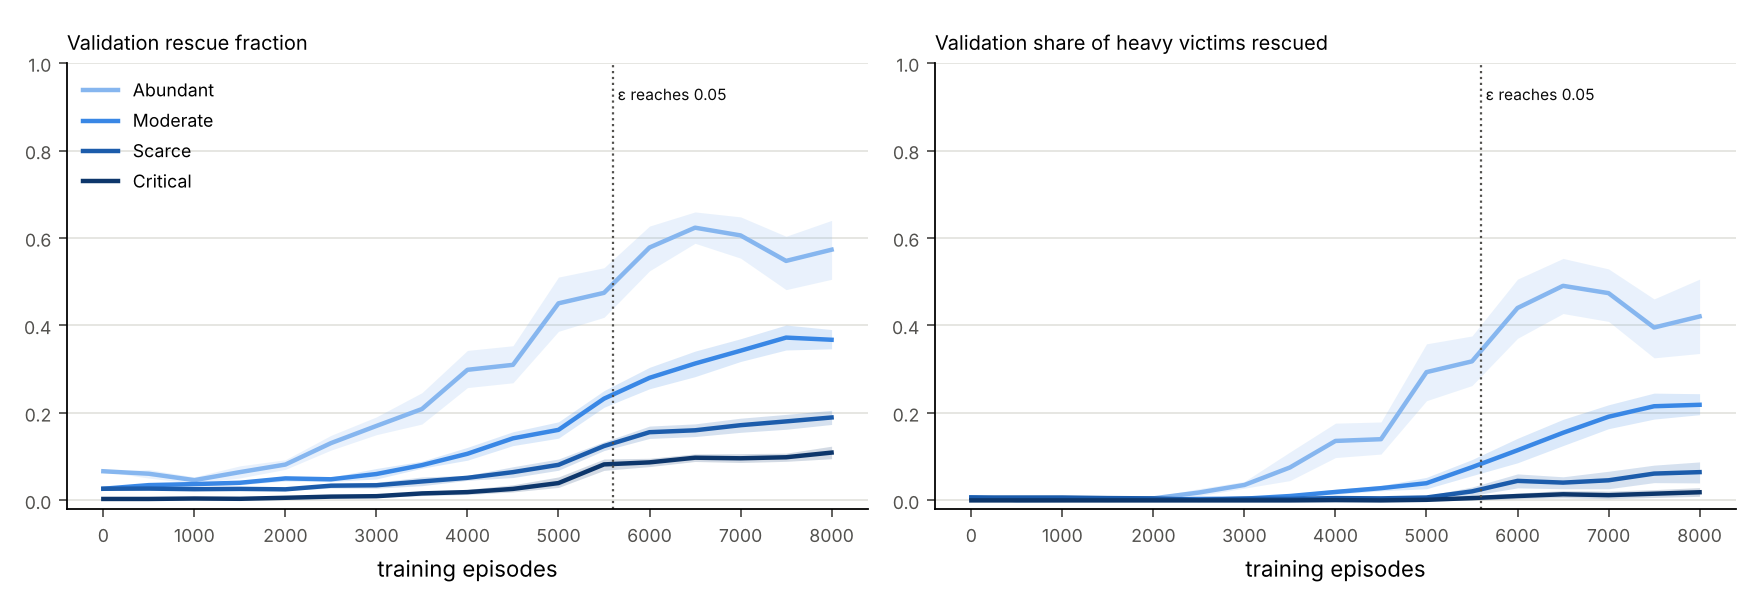
\includegraphics[width=0.8\linewidth]{fig1_learning_curves.png}
\caption{Validation learning curves (mean and 95\% CI over 10 seeds): rescue fraction (left) and share of heavy victims
rescued (right). The dotted line marks the end of $\epsilon$ decay.}
\label{fig:learning}
\end{figure}

\subsection{Scarcity and rescue performance (H1, H3)}
Scarcity lowers the rescue fraction strongly and monotonically (Table~\ref{tab:main}, Fig.~\ref{fig:rescue}):
Friedman $\chi^2(3)=30.0$, $p=1.4\times10^{-6}$, Kendall's $W=1.00$, Page $p=3.2\times10^{-14}$; in all six pairwise
comparisons every seed moves in the same direction (Holm $p=0.012$). Heavy rescues fall 26-fold ($0.422\to0.016$),
light rescues 4.5-fold. IQL beats random at every level and greedy at the three upper levels (e.g.\ $+0.117$ at
Moderate, Holm $p=0.023$), but not significantly at Critical ($+0.012$, $p=0.074$), and stays far below the cooperative
baseline. Even the oracle rescues only 62\% and 40\% at Scarce and Critical, so part of the decline is imposed by the
budget itself.

\begin{table}[h]
\centering\small
\caption{Main sweep on the 100 test maps: IQL mean [95\% CI] over 10 seeds, and baselines on the same maps.}
\label{tab:main}
\begin{tabular}{@{}lcccc@{}}
\toprule
 & Abundant (64) & Moderate (32) & Scarce (19) & Critical (13) \\
\midrule
IQL rescue fraction & 0.573 [0.517, 0.627] & 0.344 [0.319, 0.368] & 0.180 [0.166, 0.194] & 0.087 [0.076, 0.098] \\
\quad heavy victims & 0.422 [0.362, 0.483] & 0.221 [0.194, 0.248] & 0.083 [0.055, 0.107] & 0.016 [0.007, 0.026] \\
\quad light victims & 0.723 [0.672, 0.770] & 0.467 [0.440, 0.493] & 0.277 [0.254, 0.295] & 0.159 [0.140, 0.174] \\
Coverage of free cells & 0.779 & 0.591 & 0.425 & 0.327 \\
Collective return & 11.28 & 7.02 & 3.60 & 1.66 \\
Rescues per 100 units spent & 2.38 & 2.55 & 2.22 & 1.68 \\
\midrule
Random / Greedy & 0.063 / 0.465 & 0.024 / 0.227 & 0.010 / 0.123 & 0.005 / 0.075 \\
Cooperative / Oracle & 0.985 / 1.000 & 0.707 / 0.960 & 0.413 / 0.617 & 0.233 / 0.403 \\
\bottomrule
\end{tabular}
\end{table}

\begin{figure}[h]
\centering
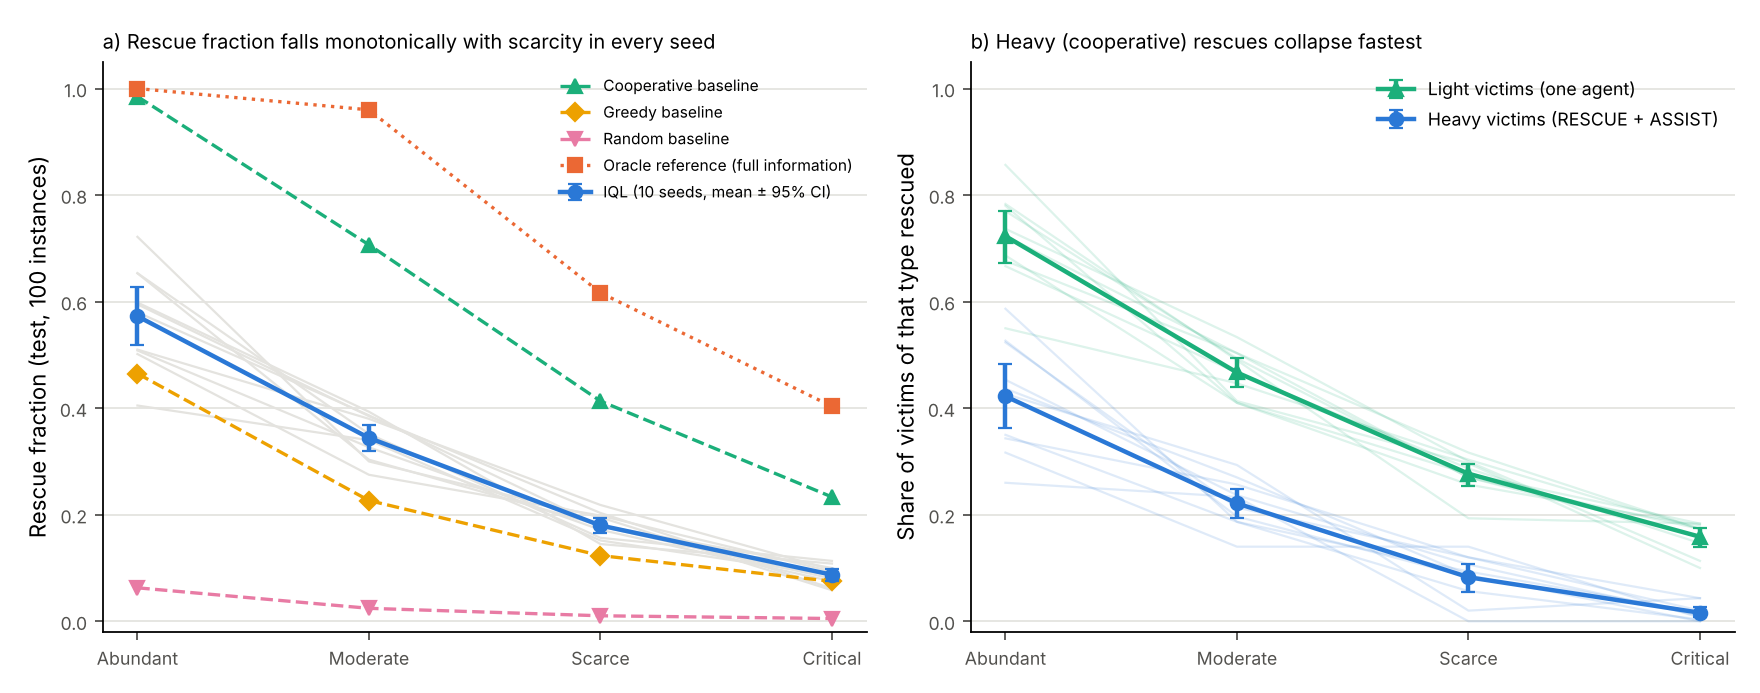
\includegraphics[width=0.95\linewidth]{fig2_exp1_rescue.png}
\caption{(a) Rescue fraction by scarcity level (thin lines: seeds; error bars: 95\% CI) with the baselines. (b) Share of
light and heavy victims rescued.}
\label{fig:rescue}
\end{figure}

\subsection{Scarcity and cooperation (H2)}
The cooperation metrics respond differently (Fig.~\ref{fig:coop}). The cooperation rate falls sharply ($0.180\to0.023$,
Holm $p=1.7\times10^{-4}$) and productive spending falls ($p=5.6\times10^{-4}$), but both depend on the number of
rescues. Search overlap with others peaks at Scarce ($0.476$ vs $0.216$ at Abundant; $p=0.025$). The metrics that do not
depend on the number of rescues show no significant trend: effective assist rate ($p=0.41$), territory division
($p=0.59$) and spending Gini ($p=0.90$). Agents do not become worse helpers when they help; they help less often
because joint rescues become rarer.

\begin{figure}[h]
\centering
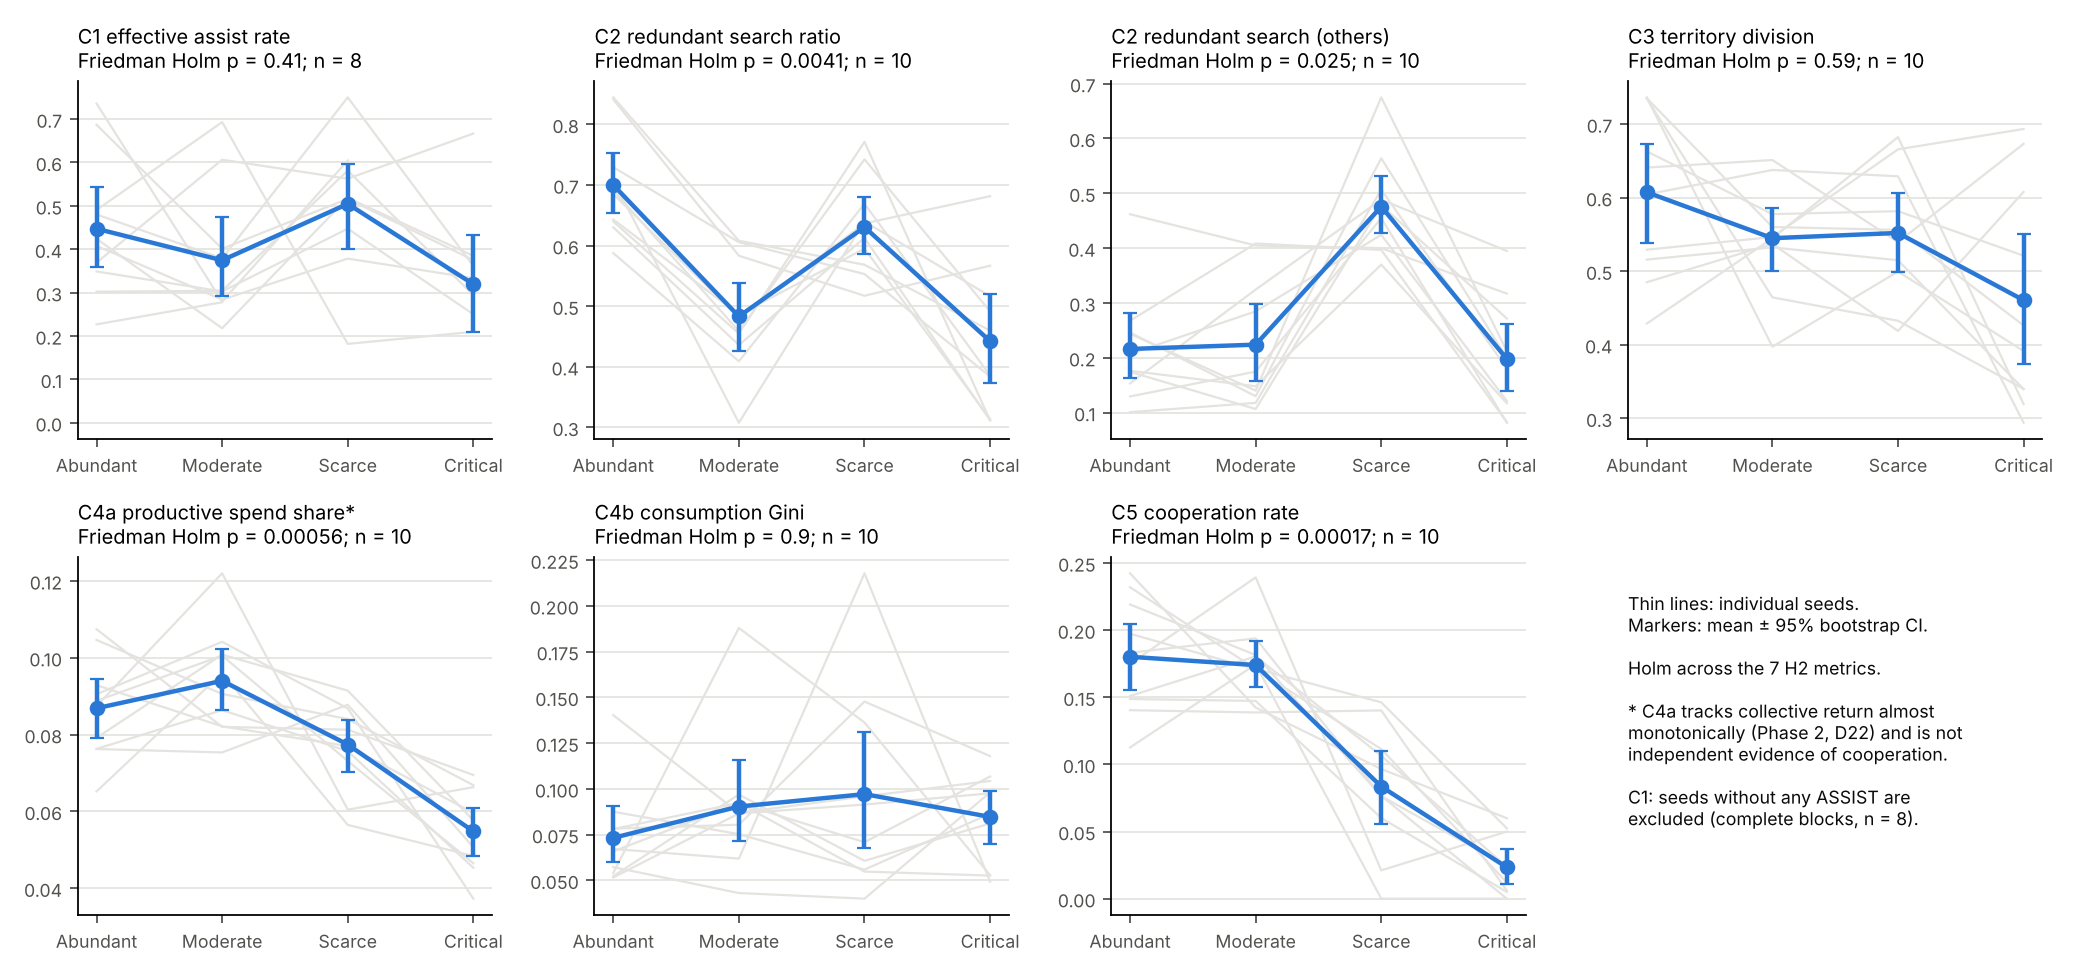
\includegraphics[width=\linewidth]{fig3_exp2_cooperation.png}
\caption{Cooperation metrics by scarcity level (thin lines: seeds; markers: mean $\pm$ 95\% CI; Friedman $p$ Holm-adjusted
across the seven metrics).}
\label{fig:coop}
\end{figure}

\subsection{Is the effect due to cooperation? (A1--A6, H4--H6)}
\textbf{Learned coordination matters} (Fig.~\ref{fig:attr}). Mismatched teams rescue less at Abundant, Moderate and
Scarce ($-0.134$, $-0.090$, $-0.043$; Holm $p\le0.027$), not significantly at Critical. Replacing one agent by a
WAIT-only agent costs $0.281$ at Abundant but $0.038$ at Critical. Jointly trained teams beat teams of solo-trained
agents at every level ($+0.471$ to $+0.081$, 10/10 seeds, Holm $p=0.008$). All these gaps shrink as budgets tighten:
the less budget there is, the less learned coordination can add. \textbf{It is not only fewer learning steps}: with as
many environment steps as Abundant (A6) the decline remains (Page $p=8\times10^{-10}$). Non-stationarity is visible
directly: between the last two checkpoints the greedy action still changes in 5--13\% of the observations agents visit (A5).

\textbf{Scarcity does not hurt more when cooperation is required (H5).} In the all-light world with the same maps and
budgets, $\RF$ falls from $0.932$ to $0.198$, more points than the heavy-victim world ($0.573\to0.087$). The
difference-in-differences at Critical is $-0.248$ $[-0.322,-0.171]$ (0/10 seeds positive, $p=0.002$): significant, but
opposite to a cooperation bottleneck. On a proportional scale the sign reverses (log-scale DiD $+0.331$, a post hoc
analysis), so we make no claim that the decline is specific to cooperation.

\begin{figure}[h]
\centering
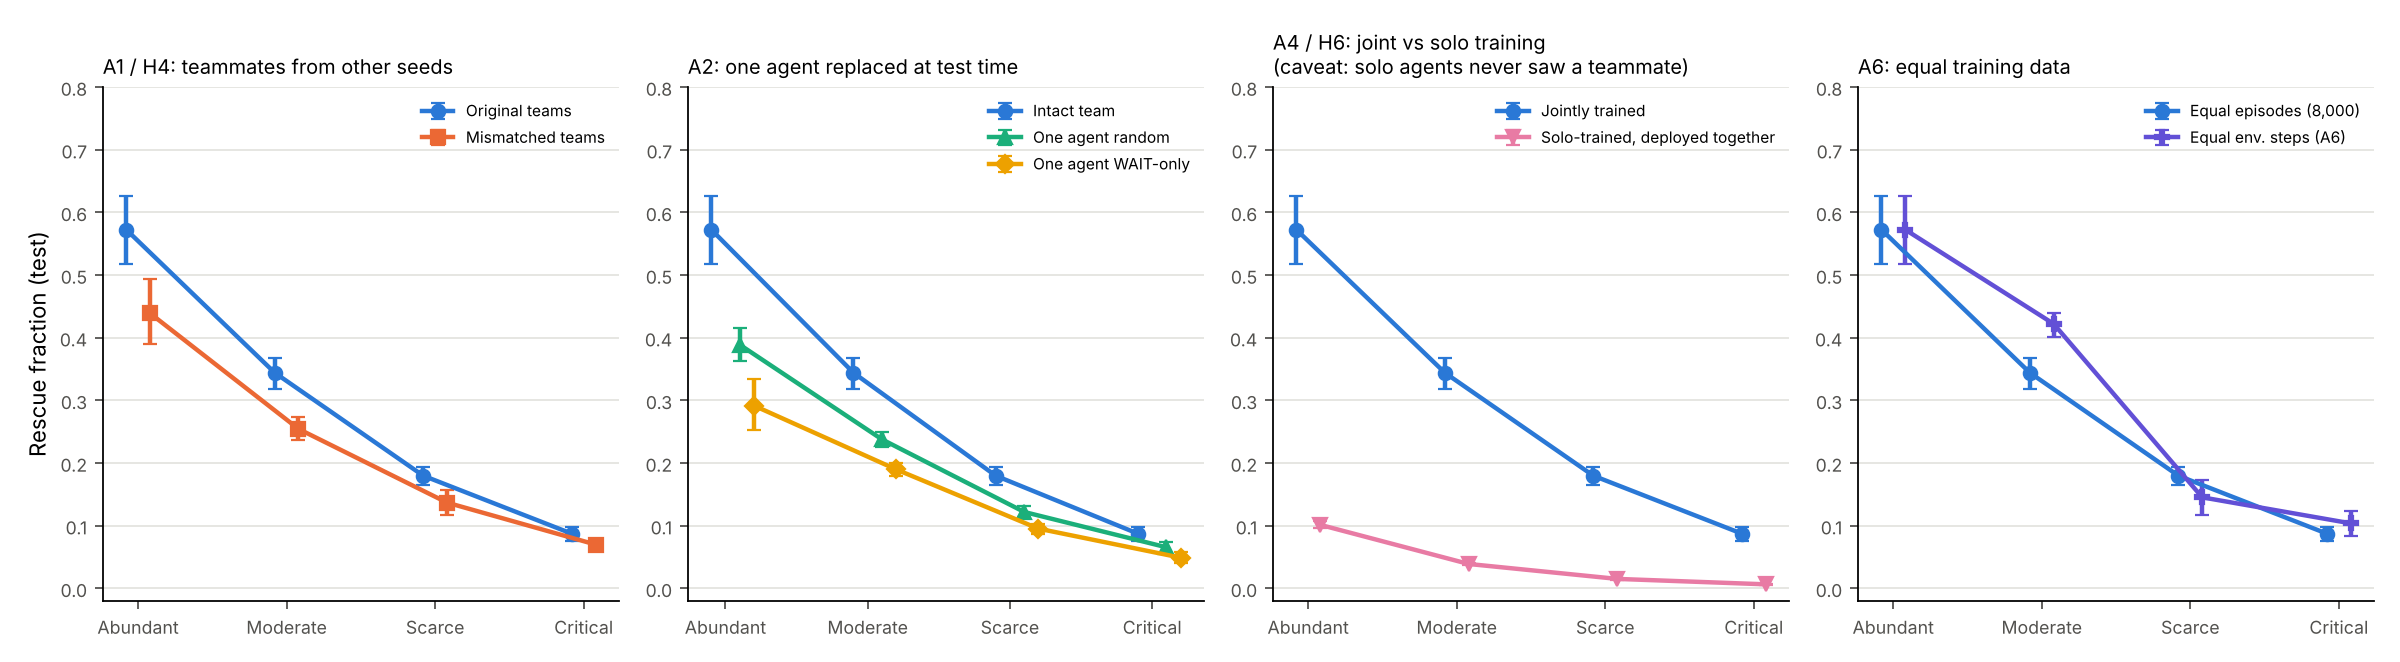
\includegraphics[width=\linewidth]{fig4_attribution.png}
\caption{Attribution checks (mean $\pm$ 95\% CI over 10 seeds): mismatched teams (A1), one agent replaced (A2), joint
vs solo training (A4), equal environment steps (A6).}
\label{fig:attr}
\end{figure}

\subsection{Individual vs collective interest, and generalisation}
Abandoned joint rescues fall from 3.34 to 0.15 per episode and duplicate light rescues from 0.36 to 0.02, mainly
because opportunities fall. The best agent's return and the team return are ranked almost identically (Spearman 0.95 at
every level), so under this reward individual and collective interest rarely diverge.
Policies are specialised to their training budget: Abundant-trained policies collapse at Critical ($0.010$ vs
$0.087$), while Moderate- and Scarce-trained ones do better there ($0.116$, $0.121$). On unseen shifted maps $\RF$ is
lower ($0.429\to0.079$) with the same ordering; on $12\times12$ maps with their own calibration the decline is the same
($0.455\to0.068$); a pooled budget raises $\RF$ slightly ($0.667\to0.129$) with an equally strong trend.

\subsection{Sensitivity to design choices (exploratory)}\label{sec:robust}
Seven further experiments each change one modelling choice and keep everything else (Table~\ref{tab:robust}).

\begin{table}[h]
\centering\small
\caption{Test $\RF$ when one design choice is changed (mean of 10 seeds; paired difference to the main block in
brackets). Page $p$: trend across levels.}
\label{tab:robust}
\begin{tabular}{@{}lccccc@{}}
\toprule
Experiment & Abundant & Moderate & Scarce & Critical & Page $p$ \\
\midrule
Main & 0.573 & 0.344 & 0.180 & 0.087 & $3\times10^{-14}$ \\
R1 budget buckets from own $b_0$ & 0.573 (+0.000) & 0.309 ($-$0.035) & 0.124 ($-$0.056) & 0.055 ($-$0.033) & $3\times10^{-14}$ \\
R2 role bit at shared cell & 0.616 (+0.043) & 0.330 ($-$0.014) & 0.169 ($-$0.011) & 0.095 (+0.008) & $3\times10^{-14}$ \\
R3 heavy credit 1.0 per role & 0.666 (+0.093) & 0.377 (+0.032) & 0.160 ($-$0.020) & 0.099 (+0.011) & $3\times10^{-14}$ \\
R4 optimistic $Q_0=2$ & 0.593 (+0.021) & 0.318 ($-$0.026) & 0.140 ($-$0.040) & 0.084 ($-$0.003) & $1\times10^{-12}$ \\
R5 dormant agents learn & 0.587 (+0.014) & 0.364 (+0.020) & 0.182 (+0.002) & 0.083 ($-$0.005) & $3\times10^{-14}$ \\
R6 trained with coop.\ partners & 0.046 ($-$0.526) & 0.034 ($-$0.310) & 0.007 ($-$0.173) & 0.018 ($-$0.069) & $6\times10^{-6}$ \\
R7 24{,}000 episodes & 0.759 (+0.186) & 0.289 ($-$0.055) & 0.176 ($-$0.004) & 0.117 (+0.030) & $1\times10^{-11}$ \\
\bottomrule
\end{tabular}
\end{table}

The decline survives every change, so none of these choices produces it. Finer budget buckets (R1) make it stronger:
agents that see their budget fall WAIT in 94\% of steps at Critical. The role bit (R2) improves assist efficiency at
Abundant (0.61 vs 0.45) but not rescues. Equal heavy credit (R3) raises heavy rescues at Abundant (0.556 vs 0.422):
the reward split affects how often heavy victims are attempted, not the trend. Optimistic values (R4) reduce waiting
without changing $\RF$, and letting dormant agents learn (R5) changes nothing. Agents trained beside scripted
cooperative teammates (R6) fail when deployed together, supporting H6 without its confound (solo agents never saw a
teammate). Three times more training (R7) raises Abundant to 0.759 but Critical only to 0.117, so the gap widens.

% =====================================================================================================================
\section{Discussion and Limitations}
% =====================================================================================================================
Scarcity strongly reduces how much independent learners rescue, and reduces cooperation-requiring rescues most.
Learned coordination is real, since mismatching, removing or separately training teammates all hurt, but its
contribution shrinks as budgets tighten. Scarcity does not break cooperation specifically: an all-light world suffers
at least as much in absolute terms, and assist efficiency, territory division and load balance do not change
significantly. All eight success criteria of the proposal are met: a tested environment, learning above random,
sensitivity to $\rho$, formal cooperation metrics, matched baselines, consistency across 10 seeds, evaluation on unseen
maps, and a reproducible pipeline.

\textbf{Limitations.} No run converged, so results describe a fixed training budget (longer training changes levels but
not the ordering). Ten seeds detect large effects only, so non-significant results are inconclusive. PSS and CR fall
partly because rescues fall. The greedy baseline is weak. $\rho$ is comparable across configurations only for
$L\ge10$, and Critical cannot go below $\rho=0.2$ without infeasible maps. The study covers one environment family,
three agents and no communication.

% =====================================================================================================================
\section{Reproducibility}
% =====================================================================================================================
Code, configurations, frozen instance lists, all training runs, raw test episodes and figures are at
\url{https://github.com/Kshitij-Giri/the-last-rescue}; the README gives the main results with plots, setup and every
command. \texttt{python scripts/run\_all.py -{}-quick} runs the whole pipeline at reduced scale and \texttt{-{}-full}
reproduces the study. All figures are produced by the repository's plotting scripts from the raw test episodes, and
\texttt{scripts/verify\_results.py} recomputes the hypothesis tests and checks every reported number against its
source file.

% =====================================================================================================================
\section{Contribution}
% =====================================================================================================================
\begin{table}[h]
\centering\small
\caption{Tasks assigned in the proposal and their completion. All members also took part in integration, debugging,
running experiments, interpreting results and proofreading.}
\label{tab:contrib}
\begin{tabularx}{\linewidth}{@{}p{2.5cm}Lp{1.2cm}@{}}
\toprule
Member & Assigned task and delivered work & Fulfilled \\
\midrule
Kshitij Suresh Giri & Coordination, formulation, integration, experimental design, report. Delivered the formal
specification and analysis plan, calibration, statistics and verification scripts, the pipeline runner and the report
build. & Yes \\
Panjari Maheshkumar Patel & Environment, maps, resources, interfaces, logging. Delivered the environment, map
generator, cost model, observation and masking, replays, the environment tests and diagrams. & Yes \\
DV Snehal & Multi-agent formulation, reward and cooperation modelling, baselines, individual--collective analysis.
Delivered the reward model, the cooperation metrics and their validation, the four baselines including the oracle,
Exp4, the association analysis and the robustness experiments R1--R7. & Yes \\
Kshitish Madbhavi & RL implementation, Q-learning pipeline, learning curves, evaluation, ablations. Delivered IQL and
training, the pilot, the 350 training runs and their evaluation, the ablations A1, A2, A4, A6 and the figures. & Yes \\
\bottomrule
\end{tabularx}
\end{table}

\begin{thebibliography}{14}
\bibitem{shoham2008} Y.~Shoham and K.~Leyton-Brown. \emph{Multiagent Systems: Algorithmic, Game-Theoretic, and Logical
Foundations}. Cambridge University Press, 2008.
\bibitem{queralta2020} J.~Pe\~na Queralta, J.~Taipalmaa, B.~C. Pullinen, V.~K. Sarker, T.~N. Gia, H.~Tenhunen,
M.~Gabbouj, J.~Raitoharju, and T.~Westerlund. Collaborative multi-robot search and rescue: Planning, coordination,
perception, and active vision. \emph{IEEE Access}, 8:191617--191643, 2020.
\bibitem{zhang2021} K.~Zhang, Z.~Yang, and T.~Ba\c{s}ar. Multi-agent reinforcement learning: A selective overview of
theories and algorithms. In \emph{Studies in Systems, Decision and Control}, volume 325, pages 321--384. Springer, 2021.
\bibitem{leibo2017} J.~Z. Leibo, V.~F. Zambaldi, M.~Lanctot, J.~Marecki, and T.~Graepel. Multi-agent reinforcement
learning in sequential social dilemmas. In \emph{Proc.\ 16th Conference on Autonomous Agents and MultiAgent Systems},
pages 464--473, 2017.
\bibitem{nguyen2018} L.~H. Nguyen, Z.~Yang, J.~Zhu, J.~Li, and F.~Jin. Coordinating disaster emergency response with
heuristic reinforcement learning. \emph{arXiv preprint arXiv:1811.05010}, 2018.
\bibitem{hickling2026} T.~Hickling, M.~Hogan, A.~Tammam, and N.~Aouf. Deep reinforcement learning based autonomous
decision-making for cooperative uncrewed aerial vehicles: A search and rescue real world application. \emph{Journal of
Field Robotics}, 43(7):4382--4401, 2026.
\bibitem{sutton2018} R.~S. Sutton and A.~G. Barto. \emph{Reinforcement Learning: An Introduction}. MIT Press, 2nd
edition, 2018.
\bibitem{watkins1992} C.~J. C.~H. Watkins and P.~Dayan. Q-learning. \emph{Machine Learning}, 8(3--4):279--292, 1992.
\bibitem{tan1993} M.~Tan. Multi-agent reinforcement learning: Independent vs.\ cooperative agents. In \emph{Proc.\ 10th
International Conference on Machine Learning}, pages 330--337. Morgan Kaufmann, 1993.
\bibitem{holm1979} S.~Holm. A simple sequentially rejective multiple test procedure. \emph{Scandinavian Journal of
Statistics}, 6(2):65--70, 1979.
\bibitem{friedman1937} M.~Friedman. The use of ranks to avoid the assumption of normality implicit in the analysis of
variance. \emph{Journal of the American Statistical Association}, 32(200):675--701, 1937.
\bibitem{page1963} E.~B. Page. Ordered hypotheses for multiple treatments: A significance test for linear ranks.
\emph{Journal of the American Statistical Association}, 58(301):216--230, 1963.
\bibitem{wilcoxon1945} F.~Wilcoxon. Individual comparisons by ranking methods. \emph{Biometrics Bulletin}, 1(6):80--83,
1945.
\bibitem{efron1979} B.~Efron. Bootstrap methods: Another look at the jackknife. \emph{The Annals of Statistics},
7(1):1--26, 1979.
\end{thebibliography}

\end{document}
